\documentclass{standalone}

\usepackage{amsmath}
\usepackage{tikz}
\usepackage{varwidth}
\usetikzlibrary{calc}
\usetikzlibrary{shapes}

 \begin{document}

 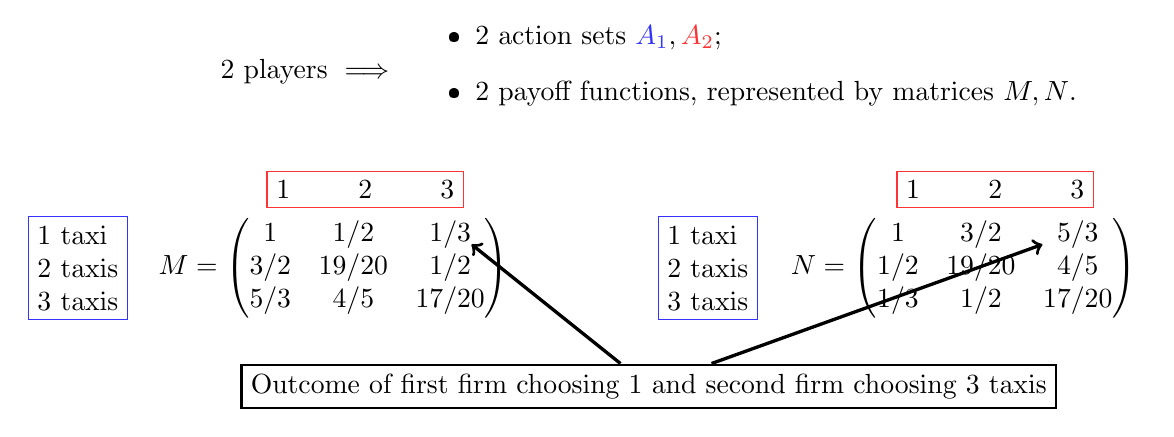
\begin{tikzpicture}

     \node (summary) at (0, 0) {2 players \(\implies\)
        {\begin{varwidth}{\linewidth}\begin{itemize}
            \item 2 action sets \({\color{blue!80}{A_1}}, \color{red!80}{A_2}\);
            \item 2 payoff functions, represented by matrices \(M, N\).
        \end{itemize}\end{varwidth}}
    };


     \node (M) at ($(summary) + (-4, -2.5)$) {
         \(M=
        \begin{pmatrix}
            1     & 1 / 2   & 1 / 3 \\
            3 / 2 & 19 / 20 & 1 / 2 \\
            5 / 3 & 4 / 5   & 17 / 20\\
        \end{pmatrix}\)
};
       \node [draw=blue!80, align=left] (A1) at ($(M) + (-3.25, 0)$) {1 taxi \\ 2 taxis \\ 3 taxis};
       \node [draw=red!80, align=left] (A2) at ($(M) + (0.4, 1)$) {1\hspace{.75cm}  2 \hspace{.75cm}3};

     \node (N) at ($(summary) + (4, -2.5)$) {
         \(N=
        \begin{pmatrix}
            1     & 3 / 2   & 5 / 3 \\
            1 / 2 & 19 / 20 & 4 / 5 \\
            1 / 3 & 1 / 2   & 17 / 20\\
        \end{pmatrix}
\)};
       \node [draw=blue!80, align=left] (A1) at ($(N) + (-3.25, 0)$) {1 taxi \\ 2 taxis \\ 3 taxis};
       \node [draw=red!80, align=left] (A2) at ($(N) + (0.4, 1)$) {1\hspace{.75cm}  2 \hspace{.75cm}3};


      \node (outcome) [draw, thick] at ($(summary) + (0, -4)$) {Outcome of first firm choosing 1 and
      second firm choosing 3 taxis};

      \draw [draw, very thick, ->] (outcome) -- ($(M) + (1.75, .3)$);
      \draw [draw, very thick, ->] (outcome) -- ($(N) + (1, .3)$);
 \end{tikzpicture}

 \end{document}
